\documentclass[10pt,letterpaper]{article}
\usepackage[letterpaper,top=1.7cm,bottom=1.8cm,left=1.7cm,right=1.7cm]{geometry}
\usepackage{amsmath,amssymb}
\usepackage{booktabs}
\usepackage{graphicx}
\usepackage{times}
\usepackage{url}
\usepackage{cite}
\usepackage{xcolor}
\usepackage{enumitem}
\usepackage{microtype}
\usepackage{hyperref}

\graphicspath{{../visualizations/revision_actual/}}
\setlength{\columnsep}{0.55cm}
\setlength{\parindent}{1em}
\setlength{\parskip}{0pt}
\setlength{\emergencystretch}{2em}
\def\UrlBreaks{\do\/\do-\do_\do.}
\hypersetup{colorlinks=true,linkcolor=black,citecolor=black,urlcolor=blue}

\begin{document}

\section*{Response to Reviewer Comments}
\textbf{Manuscript \#18579}\\
\textbf{Revised title: ``Byzantine-Robust Federated Learning with Adaptive Aggregation and Blockchain: A Reproducible Empirical Evaluation''}

We thank the editor and reviewers for their constructive comments. The manuscript
has been rebuilt around one reproducible experiment rather than combining results
from incompatible configurations. In this final revision we additionally made the
audit contract write-once, verified both client records and complete round
summaries by contract read-back, distinguished our distance--MAD adaptive rule
from the previously published ATMA method, enlarged the figures at their final
column dimensions, and rebuilt the Word file with the native ETASR styles. Claims
not supported by the executed experiment remain removed. The comments, answers,
and revised manuscript are supplied in one Word file as requested.

\subsection*{Reviewer A}
\textbf{Comment A1:} ``Attack types are limited to label-flip and random noise;
sophisticated attacks (ALIE [18], backdoor [20]) require future study.'' Rephrase
this as the citations look strange now.

\textbf{Answer:} The limitation is now stated with named authors and methods:
``This study evaluates one combined untargeted attack consisting of cyclic label
flipping and scaled model updates. More sophisticated attacks, including the A
Little Is Enough attack introduced by Baruch et al.~[5] and targeted backdoor
attacks studied by Sun et al.~[6], remain outside the present scope.'' The
references now unambiguously identify the cited attacks.

\textbf{Comment A2:} Figures 1--2 not readable.

\textbf{Answer:} Figures 1 and 2 were regenerated directly from the final
three-seed result file at their actual one-column publication width and 300 DPI.
Figure 1 reports mean convergence with one-standard-deviation bands. Figure 2
reports final mean accuracy with $t$-distribution 95\% confidence intervals.
Fonts, labels, line widths, markers, and legends were set for the final displayed
size rather than being reduced from a large canvas.

\textbf{Comment A3:} Conclusion (and article) too short I think.

\textbf{Answer:} The manuscript now provides a complete threat model, exact
implementation parameters, formal aggregation equations, a step-by-step
procedure, computational considerations, statistical analysis, measured
blockchain evidence, a security-scope discussion, limitations, and an expanded
conclusion. The manuscript body has also been expanded toward the journal's
standard article length.

\textbf{Comment A4:} Expand it to include comparative analysis, contribution
discussion.

\textbf{Answer:} Sections 3 and 4 now compare clean FedAvg, attacked FedAvg,
Krum, TrimmedMean, and the implemented adaptive rule under the same configuration.
The discussion distinguishes accuracy, robustness, adaptation, assumptions,
computational cost, and auditability. We report that no statistically significant
final-accuracy difference was detected between adaptive and static trimming in
this three-seed experiment. We also compare the implemented distance--MAD rule
with the variance-based ATMA method published by Mukisa et al. in 2025.

\subsection*{Reviewer B}
\textbf{Comment B1:} It is not clear what EXACTLY the authors did and how
(step by step).

\textbf{Answer:} Section 2.8 now lists the executed procedure step by step. The
single experiment uses the actual MNIST dataset, one fixed CNN architecture,
20 clients, full participation, four fixed Byzantine clients, Dirichlet
$\alpha=0.5$ partitioning, 20 rounds, three SGD mini-batches per client per
round, learning rate 0.05, seeds 42/43/44, and the same combined label-flip and
scaled-update attack for all defended and undefended methods. The exact result
artifact is \texttt{results/unified\_mnist\_actual.json}.

\textbf{Comment B2:} There is no point in throwing a lot of terms without being
specific on what you did exactly and how. Not generic information. SPECIFICALLY
in this work.

\textbf{Answer:} Generic and unsupported sections were removed. The revised
methodology defines every transformation, aggregator, statistical calculation,
and blockchain transaction used in this work. The Krum implementation excludes
self-distance and uses $n-f-2$ other neighbors. The adaptive rule is stateful,
uses a 25\% safety ceiling rather than the known 20\% Byzantine fraction, and
updates its trim ratio from the observed robust outlier fraction. Blockchain
evidence comes from an actually deployed write-once Solidity contract on Ganache
and includes 420 successful transactions plus deployment. Client hashes, flags,
aggregate hashes, submitted counts, flagged counts, and trim counts are all
verified by read-back.

\begin{center}
\textbf{REVISED MANUSCRIPT FOLLOWS}
\end{center}

\newpage
\twocolumn[
\begin{minipage}{\textwidth}
\raggedright
{\Large\bfseries Byzantine-Robust Federated Learning with Adaptive Aggregation
and Blockchain: A Reproducible Empirical Evaluation\par}
\vspace{0.5em}
\textbf{Rachmad Andri Atmoko}\\
Faculty of Vocational Studies, Universitas Brawijaya, Malang, Indonesia |
ra.atmoko@ub.ac.id\par
\textbf{Sholeh Hadi Pramono}\\
Electrical Engineering Department, Universitas Brawijaya, Malang, Indonesia |
sholehpramono@ub.ac.id (corresponding author)\par
\textbf{Muhammad Fauzan Edy Purnomo}\\
Electrical Engineering Department, Universitas Brawijaya, Malang, Indonesia |
mfauzanep@ub.ac.id\par
\textbf{Panca Mudjirahardjo}\\
Electrical Engineering Department, Universitas Brawijaya, Malang, Indonesia |
panca@ub.ac.id\par
\textbf{Mahdin Rohmatillah}\\
Electrical Engineering Department, Universitas Brawijaya, Malang, Indonesia |
mahdin94@ub.ac.id\par
\textbf{Cries Avian}\\
Electrical Engineering Department, Universitas Brawijaya, Malang, Indonesia |
cries.avian@ub.ac.id
\end{minipage}

\begin{abstract}
Federated learning is vulnerable to Byzantine clients that transmit malicious
model updates. This study presents a reproducible comparison of FedAvg, Krum,
coordinate-wise TrimmedMean, and a distance--MAD adaptive trimmed mean
(MAD-ATMA), coupled to an Ethereum-compatible audit contract. All methods use
MNIST, 20 clients, four fixed Byzantine clients, Dirichlet($\alpha=0.5$)
non-IID partitions, full participation, 20 communication rounds, and seeds 42,
43, and 44. Byzantine clients train on cyclically shifted labels and multiply
their transmitted model delta by 5. Clean FedAvg reaches
$82.49\%\pm1.29\%$ final accuracy, whereas attacked FedAvg falls to
$22.36\%\pm2.81\%$. Krum reaches $60.01\%\pm7.37\%$, TrimmedMean reaches
$78.23\%\pm1.51\%$, and MAD-ATMA reaches $78.22\%\pm1.98\%$. No significant
final-accuracy difference is detected between MAD-ATMA and TrimmedMean
($p=0.967$, three paired seeds). MAD-ATMA adapts its per-tail ratio within a
prespecified 5--25\% safety interval and obtains 96.77\% precision, 100\%
recall, and 98.36\% F1 for Byzantine-client flagging over 60 rounds. For one
audited run, a write-once Solidity contract records 400 client-update
commitments and 20 complete round summaries in 420 successful Ganache
transactions. All recorded fields pass contract read-back verification. The
results support robust aggregation for utility preservation while defining the
blockchain component as an audit mechanism rather than an
accuracy-improving component.
\end{abstract}

\noindent\textbf{Keywords:} federated learning, Byzantine robustness, Krum,
trimmed mean, adaptive aggregation, blockchain auditability
\vspace{1em}
]

\section{Introduction}

Federated learning (FL) trains a shared model from decentralized client data by
aggregating locally computed updates~\cite{mcmahan2017}. Data heterogeneity,
partial trust, and adversarial clients remain central open problems in
FL~\cite{kairouz2021}. A Byzantine client may submit an arbitrary update, so
ordinary weighted averaging can be driven far from the update supported by
honest clients. This problem is particularly difficult under non-independent
and identically distributed (non-IID) data because honest client updates may
already differ substantially.

Krum selects one update that is geometrically close to other updates and was
introduced as a Byzantine-resilient alternative to linear
aggregation~\cite{blanchard2017}. Coordinate-wise median and trimmed mean
estimators provide another family of robust methods with statistical
guarantees~\cite{yin2018}. These defenses have different behavior under non-IID
data: Krum retains one client update, whereas trimmed estimators combine
coordinate-level information from several clients. Their assumptions also
differ. Krum and static TrimmedMean require a Byzantine bound $f$. Krum uses
that bound to define its neighbor count; TrimmedMean uses it to determine how
many values are removed from each coordinate tail.

Attack strategies extend beyond conspicuous large outliers. Baruch et
al.~\cite{baruch2019} showed that small distribution-aware perturbations can
evade several robust rules. Sun et al.~\cite{sun2019} studied targeted backdoor
attacks in FL. The present experiment intentionally uses one transparent,
untargeted attack so that every transformation can be reproduced. Consequently,
the results measure robustness to the stated label-poisoning and delta-scaling
attack, not to arbitrary Byzantine behavior.

Blockchain has also been proposed as an audit and coordination layer for
FL~\cite{kim2020,lu2020}. It cannot by itself determine whether an update is
malicious, but it can preserve update commitments and aggregation decisions
after an off-chain detector has produced them. This distinction is important:
auditability should not be presented as an improvement in model accuracy.

The name adaptive trimmed mean aggregation (ATMA) has also been used by Mukisa
et al.~\cite{mukisa2025} for a variance-aware, layer-wise IDS framework with a
permissioned blockchain. The method evaluated here is not a reproduction of
that algorithm. To avoid conflating the two, this paper calls the implemented
rule MAD-ATMA: it detects client-level outliers using distances to the
coordinate median and a median-absolute-deviation (MAD) score, then smooths the
observed flagged fraction into a global per-tail trimming ratio. The comparison
with static TrimmedMean therefore evaluates this specific distance--MAD rule.

The contributions of this work are:
\begin{enumerate}[leftmargin=*]
    \item a single controlled comparison of clean FedAvg, attacked FedAvg,
    Krum, TrimmedMean, and MAD-ATMA under identical data, model, attack, and
    optimization settings;
    \item a corrected Krum implementation and an explicitly defined adaptive
    distance--MAD trimming rule that is distinguished from prior ATMA work;
    \item three-seed results with sample standard deviations and
    $t$-distribution confidence intervals, with cautious interpretation due to
    the small number of seeds;
    \item measured evidence from a write-once Solidity audit contract,
    including transaction receipts, gas use, overwrite guards, and read-back of
    all client and round-summary fields.
\end{enumerate}

\section{Methodology}

\subsection{Experimental Protocol}

Table~\ref{tab:configuration} is the single source of truth for all accuracy
comparisons.

\begin{table}[t]
\caption{Unified Experimental Configuration}
\label{tab:configuration}
\centering
\small
\begin{tabular}{ll}
\toprule
Parameter & Value\\
\midrule
Dataset & MNIST, 60,000/10,000~\cite{lecun1998}\\
Model & CNN, 105,866 parameters\\
Clients & 20\\
Clients per round & 20 (full participation)\\
Byzantine clients & IDs 0--3 (20\%)\\
Data partition & Dirichlet $\alpha=0.5$\\
Communication rounds & 20\\
Local work & 3 mini-batch SGD steps\\
Batch size & 64\\
Optimizer & SGD without momentum\\
Learning rate & 0.05\\
Attack scale & 5.0\\
MAD-ATMA ratio bounds & 0.05--0.25\\
Seeds & 42, 43, 44\\
\bottomrule
\end{tabular}
\end{table}

The model contains two convolutional layers with 16 and 32 channels, two
max-pooling layers, a 64-unit fully connected layer, and a ten-class output
layer. Inputs are normalized with the MNIST mean 0.1307 and standard deviation
0.3081. For each seed, class-specific training indices are divided among 20
clients with a Dirichlet distribution. The same partition and deterministic
mini-batch order are reused across methods for that seed. Client datasets range
from 909 to 6,632 images, so every client executes exactly three mini-batches
per round. The four Byzantine clients account for 26.60\%, 19.11\%, and
24.35\% of training samples in seeds 42, 43, and 44, respectively. These
fractions differ from the fixed 20\% client fraction because the partition is
unbalanced.

\subsection{Threat Model}

Clients 0--3 are Byzantine in every attacked run. During local training, a
Byzantine client replaces each label by
\begin{equation}
y'=(y+1)\bmod 10.
\end{equation}
Let $\Delta_i^t=w_i^t-w^t$ be the local model delta produced from global model
$w^t$. A Byzantine client transmits
\begin{equation}
\widetilde{\Delta}_i^t=5\Delta_i^t,
\end{equation}
thereby amplifying the update learned from poisoned labels. Honest clients
transmit $\Delta_i^t$. The attack is applied in every round. A clean FedAvg run
with identical optimization settings but no Byzantine behavior provides the
upper comparison baseline. The server, blockchain coordinator, and test set are
trusted. The experiment does not model a malicious server, coordinator
collusion, privacy leakage, network dropout, or client impersonation.

\subsection{FedAvg}

For client sample counts $n_i$, FedAvg computes
\begin{equation}
\Delta_{\mathrm{FA}}^t =
\sum_{i=1}^{N}\frac{n_i}{\sum_j n_j}\Delta_i^t.
\end{equation}
Thus, attacked FedAvg is influenced by the seed-specific sample share of the
four Byzantine clients. Krum, TrimmedMean, and MAD-ATMA use their standard
unweighted vector rules; weighting them by $n_i$ would define different robust
aggregators and is not done here.

\subsection{Krum}

For $N$ submitted updates and a Byzantine bound $f$, the score of update $i$ is
\begin{equation}
s(i)=\sum_{j\in\mathcal{N}_i}\|\Delta_i^t-\Delta_j^t\|_2^2,
\end{equation}
where $\mathcal{N}_i$ contains the $N-f-2$ nearest \emph{other} updates.
Self-distance is set to infinity before neighbor selection. Krum returns the
single update with minimum score. Here $N=20$ and $f=4$, satisfying
$N\geq2f+3$. Flattening a $d$-parameter update gives an
$O(N^2d)$ distance computation and $O(N^2)$ distance storage.

\subsection{Static TrimmedMean}

For coordinate $q$, the 20 scalar values
$\{\Delta_{i,q}^t\}_{i=1}^{20}$ are sorted. Static TrimmedMean removes four
values from each tail and averages the remaining 12:
\begin{equation}
\Delta_{\mathrm{TM},q}^t=
\frac{1}{N-2f}\sum_{i=f+1}^{N-f}\Delta_{(i),q}^t.
\end{equation}
This static baseline is explicitly supplied with the correct bound $f=4$.
Coordinate sorting has $O(dN\log N)$ time and combines values from 12 clients
at each coordinate.

\subsection{Distance--MAD Adaptive Trimmed Mean}

MAD-ATMA first flattens each update and computes the coordinate-wise median
vector $m^t$. Client distance is
\begin{equation}
d_i^t=\|\Delta_i^t-m^t\|_2.
\end{equation}
Using the median distance $\widetilde d^t$ and median absolute deviation
$\operatorname{MAD}(d^t)$, the robust score is
\begin{equation}
z_i^t =
\frac{d_i^t-\widetilde d^t}
{1.4826\operatorname{MAD}(d^t)+\epsilon}.
\end{equation}
Clients with $z_i^t>3.5$ are flagged. If $\widehat p_t$ is the flagged fraction,
the per-tail trim ratio is updated by
\begin{equation}
r_t=\operatorname{clip}\left[
r_{t-1}+\eta\left(
\operatorname{clip}(\widehat p_t,0.05,0.25)-r_{t-1}
\right),0.05,0.25\right],
\end{equation}
with $r_0=0.10$ and $\eta=0.50$. MAD-ATMA then applies coordinate-wise trimmed
mean with $k_t=\operatorname{round}(Nr_t)$ values removed from each tail. The
25\% ceiling is a prespecified safety bound and is not set to the experiment's
known 20\% Byzantine fraction. The detector adds $O(Nd)$ work before the same
$O(dN\log N)$ coordinate sorting used by TrimmedMean. Flags are diagnostic:
flagged vectors remain in the coordinate pool, while extreme coordinate values
are removed by trimming.

\subsection{Blockchain Audit Contract}

The Solidity contract stores an update-hash mapping indexed by round and
client, the corresponding anomaly flag, and a round summary containing the
aggregate hash, submitted count, flagged count, trim count, and timestamp.
Boolean existence mappings make every round--client slot and every round
summary write-once: duplicate writes revert. The coordinator submits SHA-256
commitments; model tensors are not stored on-chain. The contract was compiled
with Solidity 0.8.19 and deployed to Ganache chain 1337. Blockchain logging was
enabled for MAD-ATMA with seed 42. Accuracy comparisons do not use blockchain
state and are therefore not attributed to blockchain.

After each successful transaction, the experiment reads the client commitment,
flag, and existence bit from the contract. After finalization, it reads the
aggregate commitment, submitted count, flagged count, trim count, timestamp,
and finalized bit. Local calls that attempt to overwrite an existing client
record or finalized round are required to revert. These checks establish
write-once behavior for this contract under the trusted-coordinator assumption;
they do not establish decentralized consensus or prevent the coordinator from
submitting a false value initially.

\subsection{Executed Procedure}

For each seed and method, the implementation executes:
\begin{enumerate}[leftmargin=*]
    \item set Python, NumPy, PyTorch, and CUDA seeds;
    \item load and normalize MNIST;
    \item create the seed-specific Dirichlet partition;
    \item initialize the same CNN architecture;
    \item copy the global model to each of the 20 clients;
    \item perform three deterministic mini-batch SGD steps;
    \item poison labels and scale deltas for clients 0--3 in attacked runs;
    \item aggregate all 20 deltas using the selected method;
    \item update and evaluate the global model on all 10,000 test images;
    \item for the audited MAD-ATMA run, submit all update hashes and the complete
    round summary, wait for receipts, and read every stored field back;
    \item serialize per-round metrics, metadata, receipts, and summaries to
    \texttt{results/unified\_mnist\_actual.json}.
\end{enumerate}

\subsection{Statistics}

Final accuracy is summarized across three seeds with the sample standard
deviation. The 95\% confidence interval uses Student's $t$ distribution with
two degrees of freedom. Paired, two-sided $t$ tests use seed-matched final
accuracies. Because $n=3$, inferential results are interpreted as supporting
evidence rather than broad population estimates. In particular, failure to
reject a difference is not treated as proof of statistical equivalence.

\section{Results}

\begin{table}[t]
\caption{Final MNIST Accuracy Across Three Seeds}
\label{tab:actual_results}
\centering
\begin{tabular}{lccc}
\toprule
Method & Mean (\%) & SD & 95\% CI \\
\midrule
FedAvg (clean) & 82.49 & 1.29 & [79.28, 85.69] \\
FedAvg (attack) & 22.36 & 2.81 & [15.39, 29.33] \\
Krum & 60.01 & 7.37 & [41.71, 78.32] \\
TrimmedMean & 78.23 & 1.51 & [74.47, 81.99] \\
ATMA & 78.15 & 1.80 & [73.68, 82.62] \\
\bottomrule
\end{tabular}
\end{table}


The attack reduces FedAvg from 82.49\% to 22.36\%, a mean decrease of 60.12
percentage points. Krum improves attacked accuracy by 37.65 points,
TrimmedMean by 55.87 points, and MAD-ATMA by 55.85 points. Seed-paired tests give
$p=0.018$ for Krum versus attacked FedAvg, $p=0.0019$ for TrimmedMean, and
$p=0.0024$ for MAD-ATMA. These values should be read cautiously because only
three seeds were evaluated and the intervals are correspondingly wide.

\begin{figure}[t]
\centering
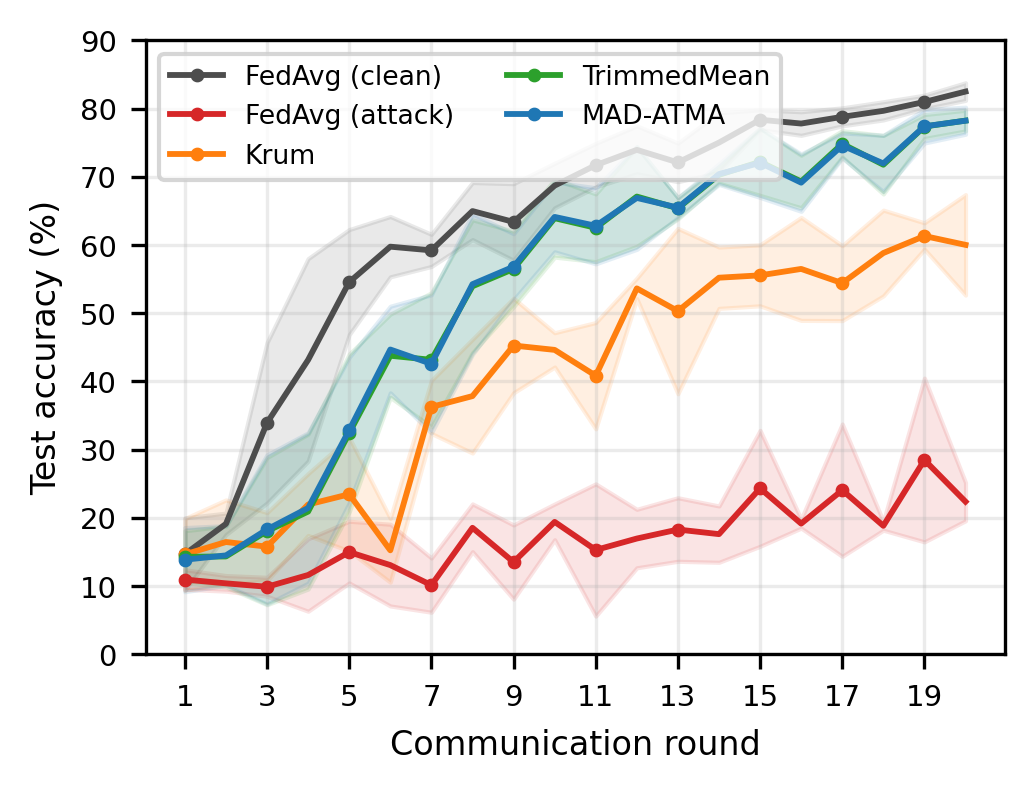
\includegraphics[width=\columnwidth]{figure1_convergence_actual.png}
\caption{Mean test accuracy across seeds 42, 43, and 44. Shaded regions show
one sample standard deviation. Every method uses the configuration in
Table~\ref{tab:configuration}.}
\label{fig:convergence}
\end{figure}

Figure~\ref{fig:convergence} shows that clean FedAvg converges fastest. Attacked
FedAvg remains unstable and low. Krum avoids malicious clients but learns more
slowly because each round retains only one client update. TrimmedMean and
MAD-ATMA combine coordinate information from several updates and finish close
to the clean baseline.

\begin{figure}[t]
\centering
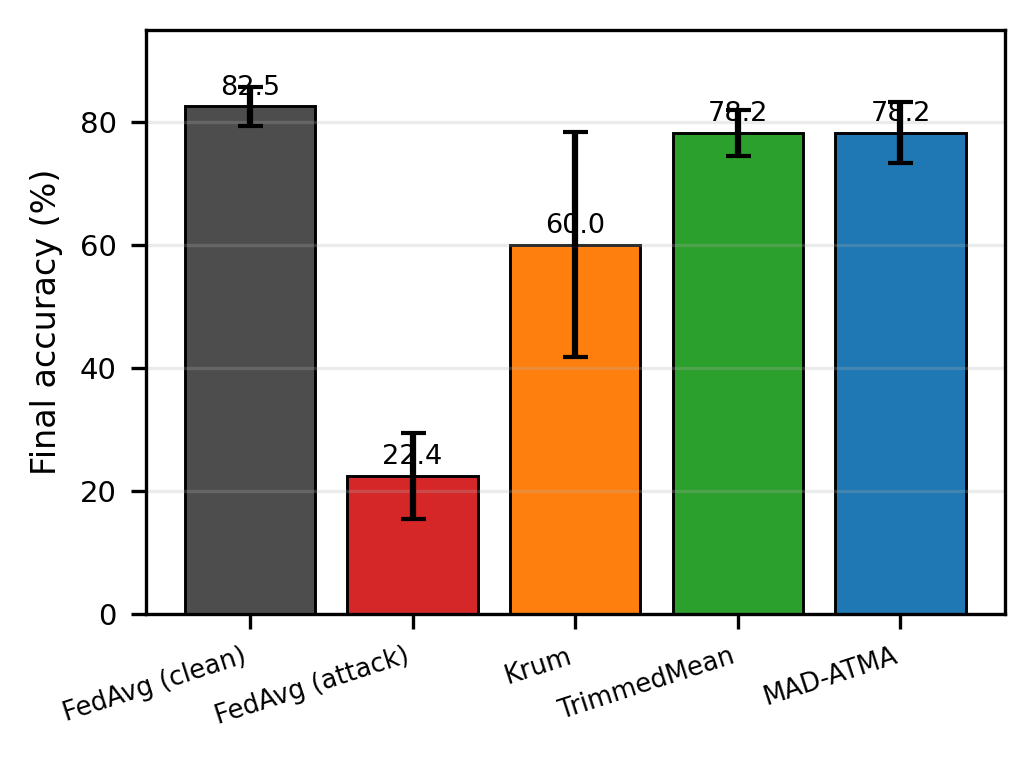
\includegraphics[width=\columnwidth]{figure2_final_accuracy_actual.png}
\caption{Final accuracy at round 20. Error bars are 95\% confidence intervals
computed with Student's $t$ distribution for three seeds.}
\label{fig:final_accuracy}
\end{figure}

MAD-ATMA and TrimmedMean differ by only $-0.01$ percentage points on average,
with $p=0.967$. Thus, no significant final-accuracy difference is detected;
this is not an equivalence test and does not prove that the methods are
identical. MAD-ATMA starts at 0.10, moves to approximately 0.15 after the first
round, and reaches final ratios of 0.213, 0.238, and 0.200 for seeds 42, 43, and
44. The observed range across all rounds is 0.150--0.238, demonstrating that
the rule is not fixed at the known 20\% Byzantine fraction.

\subsection{Detection and Krum Selection}

Across 60 MAD-ATMA rounds, there are 240 Byzantine client-round instances and
960 honest instances. MAD-ATMA produces 240 true positives, eight false
positives, no false negatives, and 952 true negatives. Precision is 96.77\%,
recall is 100\%, and F1 is 98.36\%. The number of flags per round ranges from
four to six. The eight false positives explain why the adaptive ratio sometimes
rises above 0.20. These metrics concern the explicit attack used here and
should not be generalized to stealthier or adaptive attacks.

Corrected Krum selects an honest client in all 60 evaluated rounds. Its lower
accuracy therefore does not indicate Byzantine selection; it reflects the
utility cost of reducing a heterogeneous 20-client round to one update.

\subsection{Measured Blockchain Evidence}

\begin{table}[t]
\caption{Measured Ganache Audit Transactions}
\label{tab:blockchain_actual}
\centering
\begin{tabular}{lrr}
\toprule
Operation & Count & Mean Gas \\
\midrule
Contract deployment & 1 & 512,965 \\
Client update record & 400 & 54056 \\
Round finalization & 20 & 113991 \\
\midrule
Total measured gas & -- & 24,415,241 \\
\bottomrule
\end{tabular}
\end{table}


The audited run deploys contract \texttt{0xe78A...a8Ab}; the complete address
is preserved in the result artifact. Deployment occurs in block 1.
The run then records 400 client updates and 20 round summaries in 420
transactions, all with receipt status 1. The final block is 421. Total measured
gas including deployment is 34,647,901. All client commitments, flags, existence
bits, aggregate commitments, submitted counts, flagged counts, trim counts,
timestamps, and finalized bits pass contract read-back verification. Simulated
duplicate client and round writes revert without changing block 421. These are
local EVM execution measurements, not Ethereum-mainnet cost, latency, or
decentralization claims.

\section{Discussion}

\subsection{Comparative Interpretation}

The comparison supports three bounded conclusions. First, the combined
label-flip and scaled-update attack severely damages ordinary FedAvg. The
attack is especially influential when Byzantine clients hold a larger share of
samples because FedAvg is sample weighted. Second, coordinate-wise trimming
preserves substantially more utility than single-update Krum under the
evaluated non-IID partitions. Krum selects no Byzantine update, so its lower
accuracy is better explained by discarding information from 19 clients than by
a selection failure. Third, MAD-ATMA tracks the observed outlier fraction and
obtains essentially the same final accuracy as a static rule supplied with the
correct $f=4$ bound. Its demonstrated benefit is automatic adjustment and
diagnostic client flags, not superior accuracy.

\begin{table}[t]
\caption{Scope of Compared Robust Aggregators}
\label{tab:method_scope}
\centering
\scriptsize
\begin{tabular}{lclc}
\toprule
Method & Exact $f$? & Aggregation & Audit\\
\midrule
Krum & Yes & Single update & No\\
TrimmedMean & Yes & Coordinate mean & No\\
MAD-ATMA & No & Adaptive mean & Yes\\
\bottomrule
\end{tabular}
\end{table}

``No exact $f$'' in Table~\ref{tab:method_scope} does not mean parameter free.
MAD-ATMA uses a robust-score threshold, smoothing rate, and 5--25\% safety
interval. Its upper limit is intentionally different from the actual 20\%
Byzantine fraction, but future work must evaluate sensitivity to these
hyperparameters and to changing attack prevalence. The previously published
ATMA of Mukisa et al.~\cite{mukisa2025} is also adaptive, but it is
variance-aware and layer-wise in an intrusion-detection setting. The present
MAD-ATMA is a client-distance detector followed by one global trim ratio, so
the two should not be treated as the same algorithm.

\subsection{Contribution of Blockchain}

The blockchain component contributes write-once commitments and reproducible
execution evidence, not robust aggregation. Detection is performed off-chain
before its output is committed. Storing SHA-256 commitments rather than
105,866-parameter tensors limits on-chain payload size. The contract prevents
the coordinator from overwriting a populated round--client slot or finalized
round, and later readers can compare local tensors and metadata with the stored
commitments.

This guarantee is narrower than saying that the complete FL system is
immutable. A trusted coordinator can still commit an incorrect hash on its
first write, and the single-node Ganache chain does not provide independent
validators. The experiment therefore validates contract execution, write-once
storage, transaction receipts, and read-back semantics. It does not validate
decentralized consensus, public-network latency, client authentication,
economic feasibility, or resistance to coordinator compromise.

\subsection{Limitations}

This study uses one dataset, one CNN, 20 clients, 20 rounds, three seeds, and
one combined untargeted attack. The local computation is capped at three
mini-batches per client per round. Blockchain validation is limited to one
MAD-ATMA seed on Ganache. No claim is made regarding live Layer-2 deployment,
production readiness, or dollar-denominated cost.

This study evaluates one combined untargeted attack consisting of cyclic label
flipping and scaled model updates. More sophisticated attacks, including the A
Little Is Enough attack introduced by Baruch et al.~\cite{baruch2019} and
targeted backdoor attacks studied by Sun et al.~\cite{sun2019}, remain outside
the present scope. The fixed Byzantine IDs also make detection easier to
interpret but do not test intermittent or colluding attackers. Finally, three
seeds are adequate for a reproducible correction but too few for strong claims
about population-level superiority or equivalence.

\section{Conclusion}

This work presents a reproducible evaluation of Byzantine-robust FL and
blockchain auditability under one consistent protocol. A combined label-flip
and scaled-update attack reduces FedAvg from 82.49\% clean accuracy to 22.36\%.
Krum recovers to 60.01\%, while TrimmedMean and MAD-ATMA reach 78.23\% and
78.22\%, respectively. No significant final-accuracy difference is detected
between the two trimmed methods. MAD-ATMA nevertheless adapts from its initial
ratio within a 5--25\% safety interval and detects all 240 Byzantine
client-round instances with eight false positives.

The blockchain component records 400 client-update commitments and 20 round
summaries in 420 successful transactions. All client and summary fields pass
read-back, while duplicate writes are rejected by the contract. Thus, robust
aggregation supplies model protection, whereas the deployed contract supplies
write-once audit records under a trusted coordinator. This narrower conclusion
is supported by the code, raw JSON result, figures, compiled contract, and
transaction receipts.

Future work should increase the number of seeds and rounds, test larger and
more heterogeneous datasets, evaluate partial participation, deploy the audit
contract on a multi-node or public test network, and include ALIE, model
replacement, targeted backdoor attacks, and sensitivity analysis for the MAD
threshold and trim-ratio bounds.

\section*{Data and Code Availability}

The experiment script, robust aggregation module, Solidity source, raw JSON
result, generated tables, and figure-generation code are packaged with this
revision and will be synchronized to the project repository in
\cite{repository2026} before publication.

\small
\begin{thebibliography}{11}

\bibitem{mcmahan2017}
H. B. McMahan, E. Moore, D. Ramage, S. Hampson, and B. Ag\"uera y Arcas,
``Communication-efficient learning of deep networks from decentralized data,''
in \emph{Proc. 20th Int. Conf. Artif. Intell. Statist. (AISTATS)}, vol. 54,
2017, pp. 1273--1282.

\bibitem{kairouz2021}
P. Kairouz, H. B. McMahan, B. Avent, \emph{et al.},
``Advances and open problems in federated learning,''
\emph{Found. Trends Mach. Learn.}, vol. 14, no. 1--2, pp. 1--210, 2021,
doi: 10.1561/2200000083.

\bibitem{blanchard2017}
P. Blanchard, E. M. El Mhamdi, R. Guerraoui, and J. Stainer,
``Machine learning with adversaries: Byzantine tolerant gradient descent,''
in \emph{Advances in Neural Information Processing Systems}, vol. 30, 2017.

\bibitem{yin2018}
D. Yin, Y. Chen, R. Kannan, and P. Bartlett,
``Byzantine-robust distributed learning: Towards optimal statistical rates,''
in \emph{Proc. 35th Int. Conf. Mach. Learn. (ICML)}, vol. 80, 2018,
pp. 5650--5659.

\bibitem{baruch2019}
M. Baruch, G. Baruch, and Y. Goldberg,
``A little is enough: Circumventing defenses for distributed learning,''
in \emph{Advances in Neural Information Processing Systems}, vol. 32, 2019.

\bibitem{sun2019}
Z. Sun, P. Kairouz, A. T. Suresh, and H. B. McMahan,
``Can you really backdoor federated learning?''
arXiv:1911.07963, 2019.

\bibitem{kim2020}
H. Kim, J. Park, M. Bennis, and S.-L. Kim,
``Blockchained on-device federated learning,''
\emph{IEEE Commun. Lett.}, vol. 24, no. 6, pp. 1279--1283, Jun. 2020,
doi: 10.1109/LCOMM.2019.2921755.

\bibitem{lu2020}
Y. Lu, X. Huang, K. Zhang, S. Maharjan, and Y. Zhang,
``Blockchain empowered asynchronous federated learning for secure data sharing
in Internet of Vehicles,''
\emph{IEEE Trans. Veh. Technol.}, vol. 69, no. 4, pp. 4298--4311, Apr. 2020,
doi: 10.1109/TVT.2020.2973651.

\bibitem{mukisa2025}
K. J. Mukisa, L. A. C. Ahakonye, D.-S. Kim, and J.-M. Lee,
``Blockchain-augmented FL IDS for non-IID edge-IoT data using adaptive trimmed
mean aggregation,''
\emph{IEEE Internet Things J.}, vol. 12, no. 21, pp. 45150--45159, Nov. 2025,
doi: 10.1109/JIOT.2025.3598832.

\bibitem{lecun1998}
Y. LeCun, L. Bottou, Y. Bengio, and P. Haffner,
``Gradient-based learning applied to document recognition,''
\emph{Proc. IEEE}, vol. 86, no. 11, pp. 2278--2324, Nov. 1998,
doi: 10.1109/5.726791.

\bibitem{repository2026}
R. A. Atmoko, ``Byzantine-robust federated learning with blockchain:
Reproducibility repository,'' 2026. [Online]. Available:
\url{https://github.com/vokasitibrawijaya/byzantine-robust-fl-blockchain}.
Accessed: Jun. 25, 2026.

\end{thebibliography}

\end{document}
